\providecommand{\doctitle}{Project 1: Flight Booking System}
\providecommand{\docauthor}{Nicolas Hafner, Rickert J., Peter Kr.}

\documentclass[12pt,a4paper,titlepage]{article}
\usepackage[utf8]{inputenc}
\usepackage[T1]{fontenc}
\usepackage[top=1.5cm, bottom=2.5cm, left=1cm, right=1cm]{geometry}
\usepackage{textcomp}
\usepackage{datetime}
\usepackage{fix-cm}
\usepackage{graphicx}
\usepackage{hyperref}
\usepackage{xcolor}
\usepackage{float}
\usepackage{wrapfig}
\usepackage{listings}
\usepackage{enumitem}
\newdateformat{dmny}{\monthname[\THEMONTH] \THEYEAR}
\newdateformat{dyo}{\THEYEAR}
\setlength{\headheight}{30pt}

\title{\doctitle}
\author{\docauthor}
\date{\d_mny\today}
\def\code#1{\texttt{#1}}

\begin{document}
\begin{center}{\bfseries\Huge\doctitle}\end{center}
\section{UML Model}

\begin{figure}[H]
  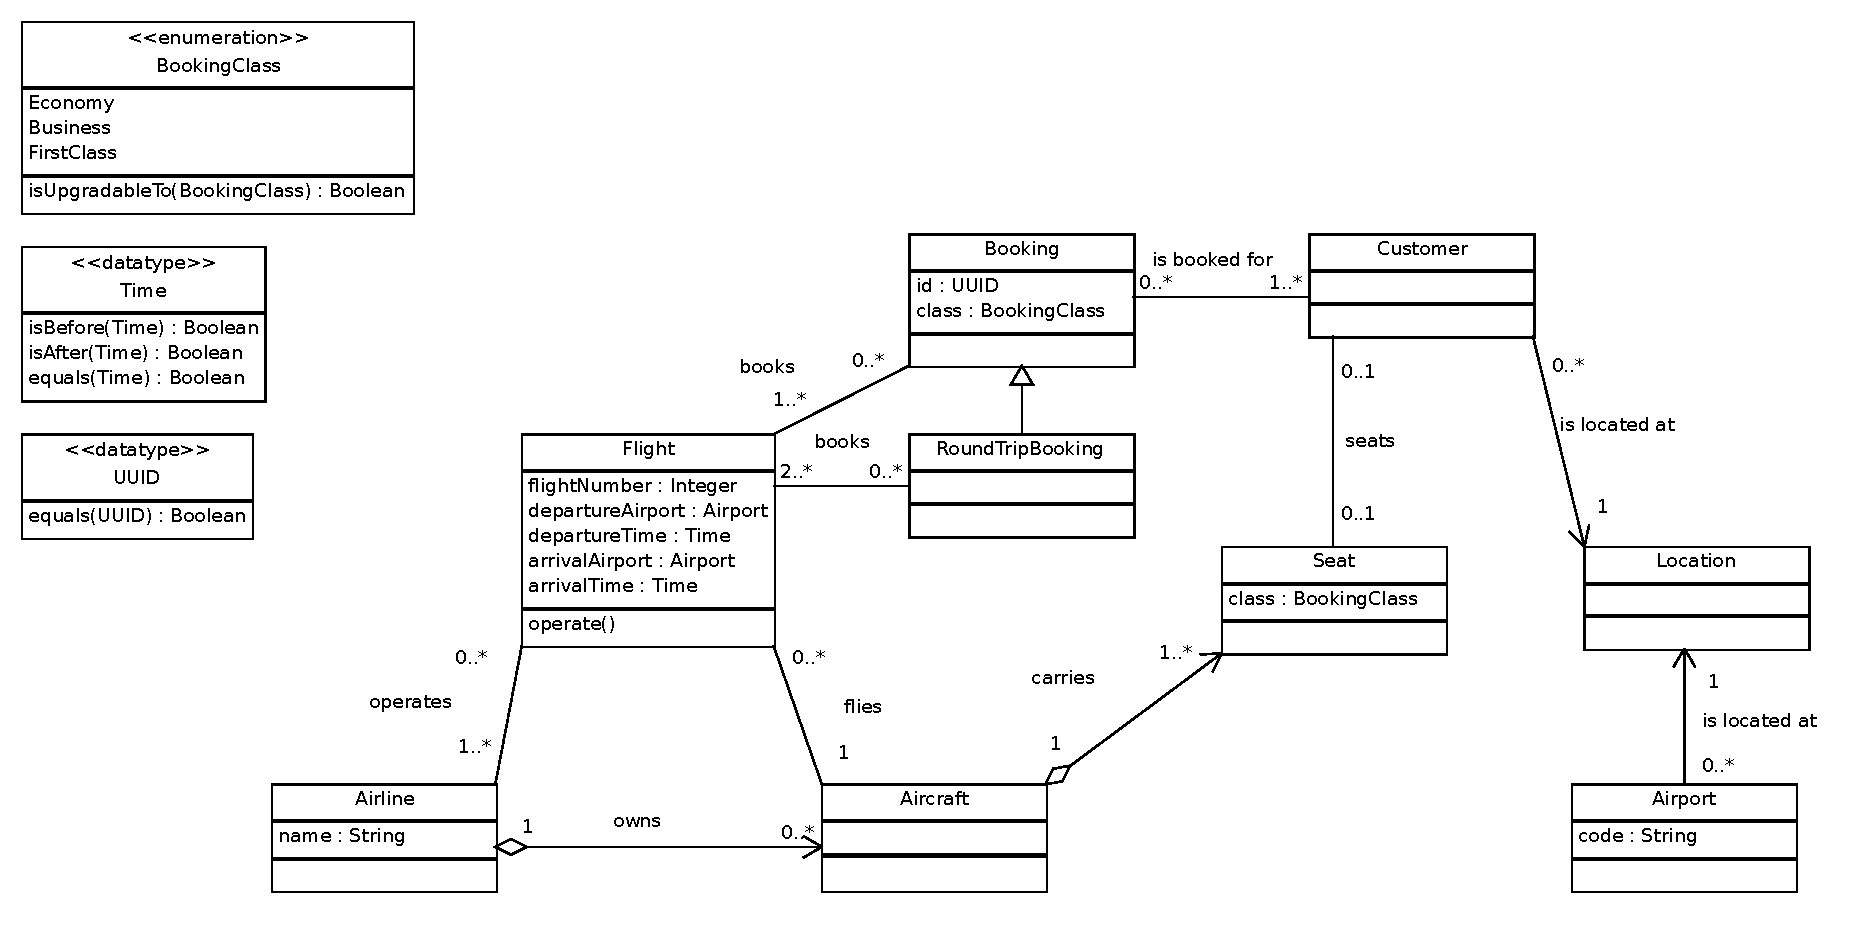
\includegraphics[width=\textwidth]{ClassDiagram}
  \caption{The UML model for the flight booking system}
\end{figure}

\section{Additional Constraints}
The following constraints are not expressible in the UML class diagram, but need to be upheld.

\begin{itemize}
\item Each \code{Flight}'s \code{departureAirport} and \code{arrivalAirport} must not match.
\item Each subsequent \code{Flight}'s \code{departureAirport} in a \code{Booking} must match the preceding \code{Flight}'s \code{arrivalAirport}.
\item Each \code{Flight} in a \code{Booking} must have a \code{departureTime} that \code{isBefore} its \code{arrivalTime}.
\item Each subsequent \code{Flight}'s \code{departureTime} in a \code{Booking} \code{isAfter} the previous \code{Flight}'s \code{arrivalTime}.
\item Each \code{Customer} associated with a \code{Booking} is tied to a \code{Seat} in each of the \code{Booking}'s \code{Flight}'s \code{Aircraft}, whose \code{class} either matches the \code{Booking}'s \code{class} or for which the \code{Booking}'s \code{class} \code{isUpgradableTo} the \code{Seat}'s \code{class}.
\item \code{Economy} \code{isUpgradableTo} \code{Business} is true.
\item \code{Business} \code{isUpgradableTo} \code{FirstClass} is true.
\item Any other combination of \code{BookingClass}es with \code{isUpgradableTo} is false.
\item A \code{Booking} may not be tied to the same \code{Customer} more than once.
\item A \code{Customer} cannot be tied to a \code{Booking} whose \code{Flight}s' \code{departureTime} \code{isBefore} and \code{arrivalTime} \code{isAfter} the \code{departureTime} of a \code{Flight} from another \code{Booking} tied to the same customer.
\item An \code{Aircraft} can only be tied to \code{Flight}s whose \code{departureTime}s and \code{arrivalTime}s do not intersect.
\item In a \code{RoundTripBooking}, the first \code{Flight}'s \code{departureAirport} must match the last \code{Flight}'s \\\code{arrivalAirport}.
\item The \code{id} of every \code{Booking} must not be \code{equal} to any other \code{Booking}'s.
\item The \code{name} of every \code{Airline} must not be \code{equal} to any other \code{Airline}'s.
\item The \code{code} of every \code{Airport} must not be \code{equal} to any other \code{Airport}'s.
\item The \code{flightNumber} of every \code{Flight} must not be \code{equal} to any other \code{Flight}'s whose \code{departureTime}s and \code{arrivalTime}s overlap.
\item Each \code{Airline} that operates a \code{Flight} has to own at least one \code{Aircraft}.
\end{itemize}

\end{document}

%%% Local Variables:
%%% mode: latex
%%% TeX-engine: luatex
%%% TeX-master: t
%%% End:
